\documentclass[a4paper, 12pt]{article}
\usepackage{comment} % enables the use of multi-line comments (\ifx \fi)
\usepackage{graphicx}
\usepackage{fullpage} % changes the margin
\usepackage{listings}
\usepackage{xparse}
\usepackage{xcolor}
\usepackage{minted}
\usepackage{amsmath}
\usepackage{varwidth}
\usepackage{tikz}

\usetikzlibrary{shapes,arrows,automata}

\tikzstyle{block} = [draw, fill=blue!20, rectangle, 
    minimum height=3em, minimum width=6em]
\tikzstyle{sum} = [draw, fill=blue!20, circle, node distance=1cm]
\tikzstyle{input} = [coordinate]
\tikzstyle{output} = [coordinate]
\tikzstyle{pinstyle} = [pin edge={to-,thin,black}]

\NewDocumentCommand{\codeword}{v}{%
\texttt{\textcolor{blue}{#1}}%
}

\newcommand{\block}[1]{%
  \begingroup
  \setlength{\fboxsep}{0pt}%
  \vrule width0pt height \blockdim
  \ooalign{%
    \framebox[\blockdim]{\rule{0pt}{\blockdim}}\cr
    \hidewidth\raisebox{0.5\dimexpr\blockdim-\height}{\raisebox{\depth}{#1}}\hidewidth\cr
  }%
  \endgroup
}
\newcommand{\joinblocks}{\unskip\kern-\fboxrule\ignorespaces}
\newenvironment{blocks}[1][1cm]
 {\begin{varwidth}{\textwidth}\setlength{\blockdim}{#1}\makeblocks}
 {\end{varwidth}}
\newcommand{\makeblocks}{%
  \begingroup\lccode`~=`&\lowercase{\endgroup\let~}\joinblocks
  \catcode`\&=\active
  \baselineskip=0pt
  \lineskiplimit=\maxdimen
  \lineskip=0pt
  \centering
}
\newlength{\blockdim}

\begin{document}
% Header
\noindent
\LARGE\textbf{Intrastellar} \hfill \\
\newline
\large\textbf{Preliminary Design Report} \hfill \textbf{Zach Schuermann} \\
\normalsize ECE 4273-001 \hfill 112944063 \\
Dr. Erik Petrich \hfill Date: 04/16/19 

\section*{Project Objectives}
The ultimate goal for this project is to create a Galaga-like game implemented on an LPC1769 with a Playstation 2 controller for user input/control and a 480x800 LCD display.

\section*{Solution Design}
add more

\begin{center}
  \begin{tabular}{ |c|c|c| }
    \hline
    \textbf{Component} & \textbf{Description} & \textbf{Points} \\
    \hline
    \hline
    Game Type & Animated real-time game (objects continuously in motion) & 2 \\
    \hline
    Display & Use a graphical LCD for output  & 2 \\
    \hline
    Input & Use a game controller with a serial interface (Playstation 2) & 0.5 \\ 
    \hline
    Sound & Use D-to-A to generate a sine wave based sound effect  & 1 \\
    \hline
    Other & Use non-volatile memory (EEPROM  to retain high score table) & 0.5 \\ 
    \hline
    Total & & 6 \\ 
    \hline
  \end{tabular}
\end{center}

\begin{figure}[h!]
  \centering
  \includegraphics[scale=.6]{screen2.png}
  \caption{659 Hz doorbell signal}
  \label{fig:screen1}
\end{figure}

\begin{figure}[h!]
  \centering
  \includegraphics[scale=.6]{screen1.png}
  \caption{523 Hz doorbell signal}
  \label{fig:screen2}
\end{figure}

\section*{Hardware Design}
The hardware was relatively straightforward. In the case of choosing load resistance for the phototransistor, trial and error was used (within the reasonable guesses from the component's documentation) such that there was enough fluctuation to have a discernible (and reliable) difference between the two different states (light and dark). Noise was mitigated through the use of capacitors on the power rails of integrated circuits as well as between the speaker load and the opamp. 

\section*{Software Design}
The software included the steps necessary to speed up the CPU clock through using an internal phase-locked loop. Further discussion is deferred as this was covered in Assignment 3. The remainder of the software implements simple digital logic and interfacing with the DAC and ADC subsystems. The main 'loop' for the program simply reads from the ADC to retrieve the light measurement, and lights or dims the LED accordingly. In the same loop, a state which synthesizes the doorbell sounds is triggered through pressing the switch. Most of the functionality is decomposed in discrete functions such as \codeword{clock_setup()} for raising the CPU clock, or \codeword{ding()} and \codeword{dong()} for implementing the waveform synthesis. 

\section*{Final Solution Details}
The final circuit schematic is included below: 
\begin{figure}[h!]
  \centering
  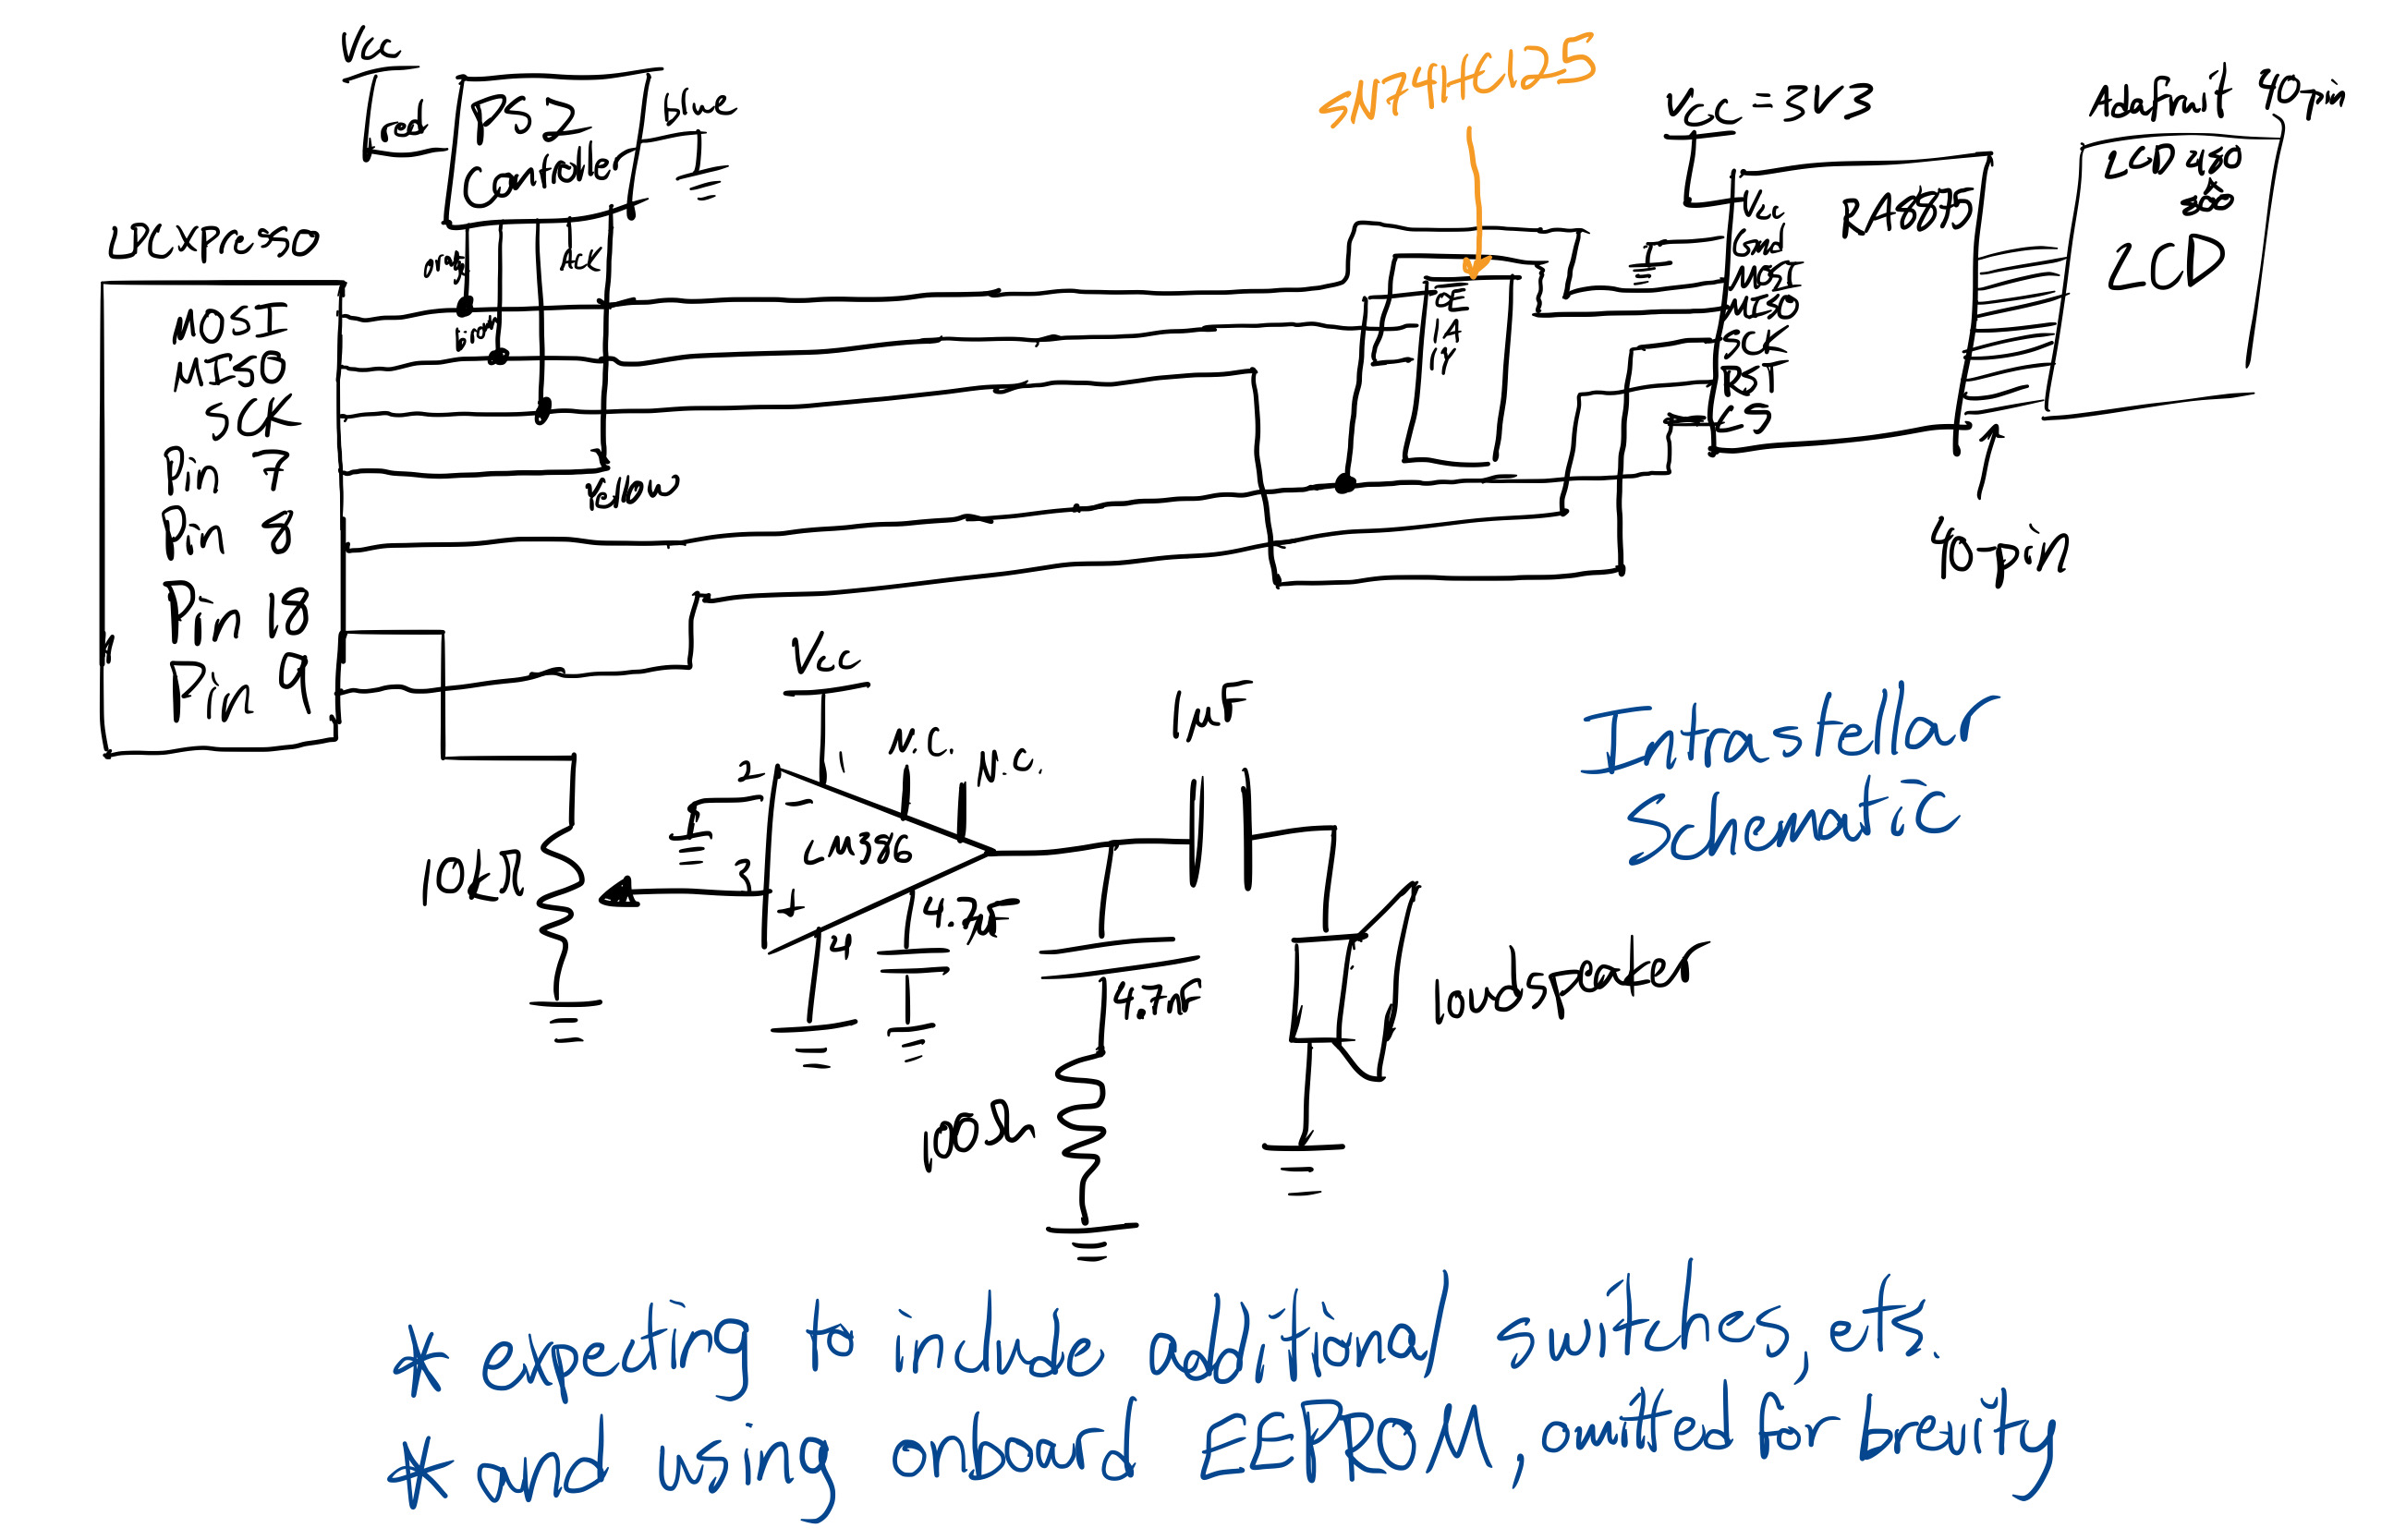
\includegraphics[scale=.2]{schematic.png}
  \caption{Circuit Schematic}
  \label{fig:schematic}
\end{figure}

The completed source code is included below: \newline
\newline
\newline
\begin{minted}{c}


\end{minted}

\section*{Discussion}
Floating point numbers were utilized for the generation of the sinusoid. That is, floating-point sine calculations occurred every iteration of the program. This was likely a rather poor performing implementation. The solution could be further improved through the use of integer calculations and even precomputing the values which needed to be written to the analog output thereby reducing the calculation to constant time lookup. 
\end{document}
